\subsubsection{Estimaci\'on de la Tasa de Descuento Ke.}

Cuanto mayor sea el riesgo sistem\'atico de una acci\'on, m\'as elevado ser\'a el rendimiento que los inversionistas esperar\'an de los t\'itulos accionarios. Con la finalidad de estimar una tasa de descuento apropiada en pesos, en t\'erminos nominales y despu\'es de impuestos, se utilizaron los siguientes insumos para determinar el valor de la \gls{wacc}:\\


\textcolor{principal}{Tasa libre de riesgo (Rf).} Se basa en el rendimiento de los bonos gubernamentales, en este caso, se tom\'o en rendimiento del \textcolor{principal}{\rfBase}, con el siguiente resultado:

\begin{figure}[H]
\centering
La tasa libre de riesgo obtenida es de \textbf{\rfValor\%} \includegraphics[width=9cm]{../0.imagenes/rf}
\end{figure}

\gls{beta}. Con la finalidad de determinar el factor \gls{beta} apropiado para el negocio, se consider\'o una muestra de mercado de \glspl{leveredbeta} de empresas comparables al negocio valuado:

\espacio{4cm}
\begin{figure}[H]
\centering
\includegraphics[width=6cm]{../0.imagenes/beta_1}\\
\end{figure}


\begin{figure}[H]
\centering
\includegraphics[width=9cm]{../0.imagenes/beta_2}
\end{figure}

La beta apalancada de sector que corresponde a la empresa es de \textcolor{principal}{\textbf{\valorBeta x }(media aritmética)}\\

La Beta desapalancada del sector es de \textcolor{principal}{\betaDesapalancada x} la cual, al incluirse el efecto de los impuestos y la proporción de deuda-capital de la empresa analizada, muestra un resultado de \textcolor{principal}{\betaReapalancada x} como beta reapalancada ({\textitt Relevered Beta}).\\


\textcolor{principal}{Muestra de mercado de la estructura de Deuda/Capital del sector (D/E):}

\begin{figure}[H]
\centering
\includegraphics[width=12cm]{../0.imagenes/DE}
\end{figure}

\textcolor{principal}{Muestra de mercado de la tasa efectiva de impuestos a la utilidad (ETR\%) del sector:}

\begin{figure}[H]
\centering
\includegraphics[width=12cm]{../0.imagenes/ETR}
\end{figure}

F\'ormula de BETA Apalancada:
\begin{figure}[H]
\centering

\includegraphics[width=8cm]{\rutaImagenes/beta_apalancada}
\end{figure}

El valuador llev\'o a cabo la estimaci\'on del pron\'ostico de BETA desapalancada al negocio, habiendo aplicado a la proporci\'on de deuda/capital del sujeto el promedio de la muestra y la tasa fiscal efectiva del sector (ETR\footnote{Efective Tax Rate}); con un resultado de 1.16x.\\

F\'ormula de BETA Reapalancada:\\

\begin{figure}[H]
\centering

\includegraphics[width=8cm]{\rutaImagenes/beta_reapalancada}
\end{figure}

Una vez obtenido el indicador de BETA desapalancada del sector, el valuador llev\'o a cabo la estimaci\'on del pron\'ostico de BETA reapalancada al negocio sujeto de valuaci\'on, habiendo aplicado a la proporci\'on de deuda/capital del sujeto la mediana\footnote{Conforme a la aplicaci\'on del rango intercuartil como medida de estandarizaci\'on}  de la muestra del sector y la tasa fiscal de M\'exico (MTR\footnote{Marginal Tax Rate}), con un resultado de 1.49x.\\

\newpage



\textcolor{principal}{Prima de riesgo del mercado de capitales}. Se obtuvo del promedio hist\'orico de la diferencia de rendimientos o ``spread'' entre el mercado accionario \mercadoAccionario mediante el indicador conocido como el \gls{erp} (enterprise risk premium).\\

\begin{figure}[H]
\centering
La prima de riesgo de mercado (\gls{erp}) es de \textbf{\textcolor{principal}{\erpValor\%}} 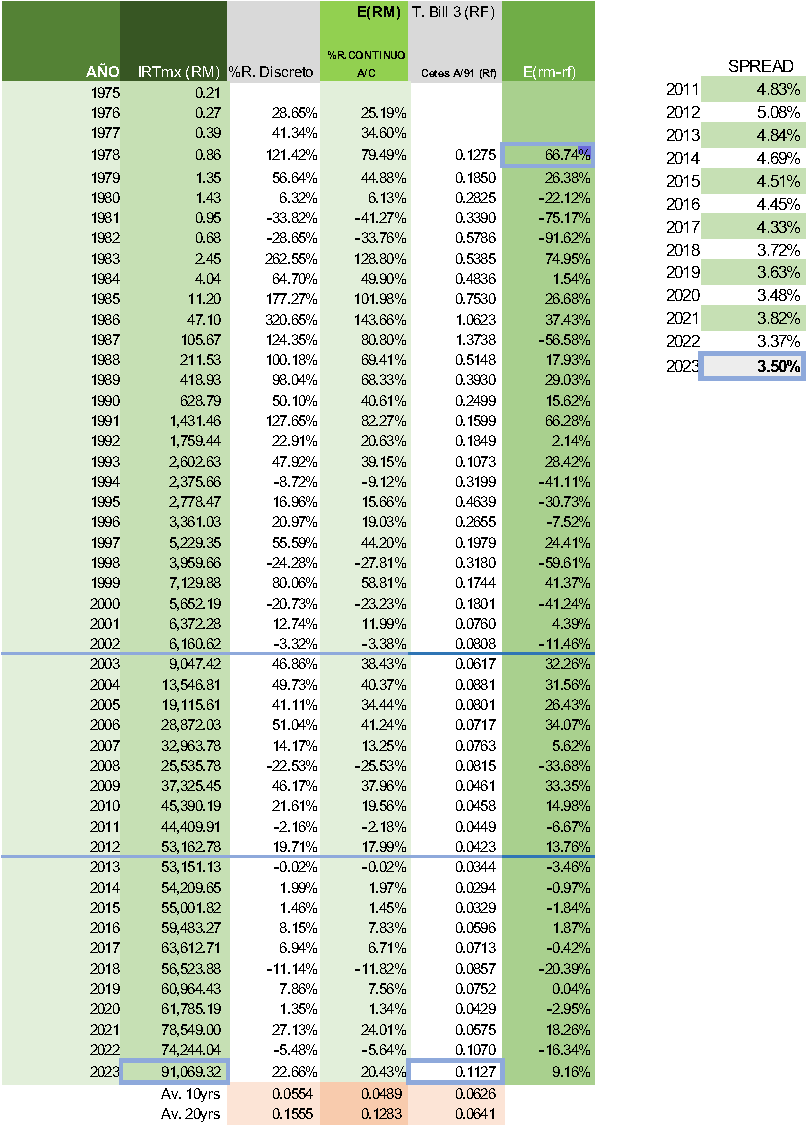
\includegraphics[width=5cm]{../0.imagenes/erp}
\end{figure}

\textcolor{principal}{Riesgo Pa\'is (\gls{crp}).} Corresponde al riesgo pa\'is de M\'exico, seg\'un indicador de JP Morgan. Se considera un pron\'ostico para la prima de riesgo adicional de \crpValor{} puntos base.

\begin{figure}[H]
\centering
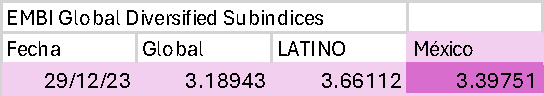
\includegraphics[width=8cm]{../0.imagenes/crp}
\end{figure}

Estimaci\'on del costo de capital (\gls{ke}), con un resultado de \textcolor{principal}{\keValor\%.}

\begin{figure}[H]
\centering
\includegraphics[width=10cm]{../0.imagenes/ke}
\end{figure}

%A su vez, se llev\'o a cabo un pron\'ostico de crecimiento para la capitalizaci\'on, tomando en cuenta la Encuesta de especialistas de Banxico, la cual muestra los siguientes resultados:
%
%\begin{figure}[H]
%\centering
%\includegraphics[width=15cm]{../0.imagenes/banxico}
%\end{figure}
%
%En vista de lo anterior, se estableci\'o un pron\'ostico de \textcolor{principal}{tasa neta} de capitalizaci\'on, la cual muestra los siguientes resultados:
%
%\begin{figure}[H]
%\centering
%\includegraphics[width=8cm]{../0.imagenes/tasa_neta}
%\end{figure}

\textcolor{principal}{Costo de la deuda (\gls{kd}).} Para determinar la tasa \gls{wacc}, se consider\'o el costo impl\'icito de la deuda de la organizaci\'on, de acuerdo a par\'ametros de mercado de empresas similares:

\begin{figure}[H]
\centering
\includegraphics[width=10cm]{../0.imagenes/kd}
\end{figure}

\textcolor{principal}{C\'alculo del \gls{wacc}.} Como resultado de las consideraciones anteriores, se estima una \gls{wacc} en t\'erminos nominales y despu\'es de impuestos de \textcolor{principal}{\waccValor\%}.\\

\begin{figure}[H]
\centering
\includegraphics[width=12cm]{../0.imagenes/calculo_wacc}
\end{figure}

